\documentclass[1p]{elsarticle_modified}
%\bibliographystyle{elsarticle-num}

%\usepackage[colorlinks]{hyperref}
%\usepackage{abbrmath_seonhwa} %\Abb, \Ascr, \Acal ,\Abf, \Afrak
\usepackage{amsfonts}
\usepackage{amssymb}
\usepackage{amsmath}
\usepackage{amsthm}
\usepackage{scalefnt}
\usepackage{amsbsy}
\usepackage{kotex}
\usepackage{caption}
\usepackage{subfig}
\usepackage{color}
\usepackage{graphicx}
\usepackage{xcolor} %% white, black, red, green, blue, cyan, magenta, yellow
\usepackage{float}
\usepackage{setspace}
\usepackage{hyperref}

\usepackage{tikz}
\usetikzlibrary{arrows}

\usepackage{multirow}
\usepackage{array} % fixed length table
\usepackage{hhline}

%%%%%%%%%%%%%%%%%%%%%
\makeatletter
\renewcommand*\env@matrix[1][\arraystretch]{%
	\edef\arraystretch{#1}%
	\hskip -\arraycolsep
	\let\@ifnextchar\new@ifnextchar
	\array{*\c@MaxMatrixCols c}}
\makeatother %https://tex.stackexchange.com/questions/14071/how-can-i-increase-the-line-spacing-in-a-matrix
%%%%%%%%%%%%%%%

\usepackage[normalem]{ulem}

\newcommand{\msout}[1]{\ifmmode\text{\sout{\ensuremath{#1}}}\else\sout{#1}\fi}
%SOURCE: \msout is \stkout macro in https://tex.stackexchange.com/questions/20609/strikeout-in-math-mode

\newcommand{\cancel}[1]{
	\ifmmode
	{\color{red}\msout{#1}}
	\else
	{\color{red}\sout{#1}}
	\fi
}

\newcommand{\add}[1]{
	{\color{blue}\uwave{#1}}
}

\newcommand{\replace}[2]{
	\ifmmode
	{\color{red}\msout{#1}}{\color{blue}\uwave{#2}}
	\else
	{\color{red}\sout{#1}}{\color{blue}\uwave{#2}}
	\fi
}

\newcommand{\Sol}{\mathcal{S}} %segment
\newcommand{\D}{D} %diagram
\newcommand{\A}{\mathcal{A}} %arc


%%%%%%%%%%%%%%%%%%%%%%%%%%%%%5 test

\def\sl{\operatorname{\textup{SL}}(2,\Cbb)}
\def\psl{\operatorname{\textup{PSL}}(2,\Cbb)}
\def\quan{\mkern 1mu \triangleright \mkern 1mu}

\theoremstyle{definition}
\newtheorem{thm}{Theorem}[section]
\newtheorem{prop}[thm]{Proposition}
\newtheorem{lem}[thm]{Lemma}
\newtheorem{ques}[thm]{Question}
\newtheorem{cor}[thm]{Corollary}
\newtheorem{defn}[thm]{Definition}
\newtheorem{exam}[thm]{Example}
\newtheorem{rmk}[thm]{Remark}
\newtheorem{alg}[thm]{Algorithm}

\newcommand{\I}{\sqrt{-1}}
\begin{document}

%\begin{frontmatter}
%
%\title{Boundary parabolic representations of knots up to 8 crossings}
%
%%% Group authors per affiliation:
%\author{Yunhi Cho} 
%\address{Department of Mathematics, University of Seoul, Seoul, Korea}
%\ead{yhcho@uos.ac.kr}
%
%
%\author{Seonhwa Kim} %\fnref{s_kim}}
%\address{Center for Geometry and Physics, Institute for Basic Science, Pohang, 37673, Korea}
%\ead{ryeona17@ibs.re.kr}
%
%\author{Hyuk Kim}
%\address{Department of Mathematical Sciences, Seoul National University, Seoul 08826, Korea}
%\ead{hyukkim@snu.ac.kr}
%
%\author{Seokbeom Yoon}
%\address{Department of Mathematical Sciences, Seoul National University, Seoul, 08826,  Korea}
%\ead{sbyoon15@snu.ac.kr}
%
%\begin{abstract}
%We find all boundary parabolic representation of knots up to 8 crossings.
%
%\end{abstract}
%\begin{keyword}
%    \MSC[2010] 57M25 
%\end{keyword}
%
%\end{frontmatter}

%\linenumbers
%\tableofcontents
%
\newcommand\colored[1]{\textcolor{white}{\rule[-0.35ex]{0.8em}{1.4ex}}\kern-0.8em\color{red} #1}%
%\newcommand\colored[1]{\textcolor{white}{ #1}\kern-2.17ex	\textcolor{white}{ #1}\kern-1.81ex	\textcolor{white}{ #1}\kern-2.15ex\color{red}#1	}

{\Large $\underline{12n_{0329}~(K12n_{0329})}$}

\setlength{\tabcolsep}{10pt}
\renewcommand{\arraystretch}{1.6}
\vspace{1cm}\begin{tabular}{m{100pt}>{\centering\arraybackslash}m{274pt}}
\multirow{5}{120pt}{
	\centering
	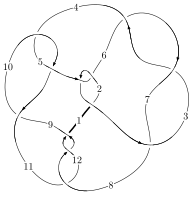
\includegraphics[width=112pt]{../../../GIT/diagram.site/Diagrams/png/2418_12n_0329.png}\\
\ \ \ A knot diagram\footnotemark}&
\allowdisplaybreaks
\textbf{Linearized knot diagam} \\
\cline{2-2}
 &
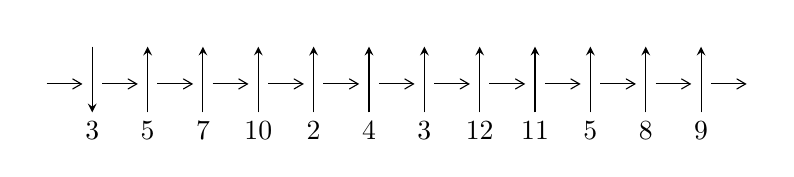
\begin{tikzpicture}[x=20pt, y=17pt]
	% nodes
	\node (C0) at (0, 0) {};
	\node (C1) at (1, 0) {};
	\node (C1U) at (1, +1) {};
	\node (C1D) at (1, -1) {3};

	\node (C2) at (2, 0) {};
	\node (C2U) at (2, +1) {};
	\node (C2D) at (2, -1) {5};

	\node (C3) at (3, 0) {};
	\node (C3U) at (3, +1) {};
	\node (C3D) at (3, -1) {7};

	\node (C4) at (4, 0) {};
	\node (C4U) at (4, +1) {};
	\node (C4D) at (4, -1) {10};

	\node (C5) at (5, 0) {};
	\node (C5U) at (5, +1) {};
	\node (C5D) at (5, -1) {2};

	\node (C6) at (6, 0) {};
	\node (C6U) at (6, +1) {};
	\node (C6D) at (6, -1) {4};

	\node (C7) at (7, 0) {};
	\node (C7U) at (7, +1) {};
	\node (C7D) at (7, -1) {3};

	\node (C8) at (8, 0) {};
	\node (C8U) at (8, +1) {};
	\node (C8D) at (8, -1) {12};

	\node (C9) at (9, 0) {};
	\node (C9U) at (9, +1) {};
	\node (C9D) at (9, -1) {11};

	\node (C10) at (10, 0) {};
	\node (C10U) at (10, +1) {};
	\node (C10D) at (10, -1) {5};

	\node (C11) at (11, 0) {};
	\node (C11U) at (11, +1) {};
	\node (C11D) at (11, -1) {8};

	\node (C12) at (12, 0) {};
	\node (C12U) at (12, +1) {};
	\node (C12D) at (12, -1) {9};
	\node (C13) at (13, 0) {};

	% arrows
	\draw[->,>={angle 60}]
	(C0) edge (C1) (C1) edge (C2) (C2) edge (C3) (C3) edge (C4) (C4) edge (C5) (C5) edge (C6) (C6) edge (C7) (C7) edge (C8) (C8) edge (C9) (C9) edge (C10) (C10) edge (C11) (C11) edge (C12) (C12) edge (C13) ;	\draw[->,>=stealth]
	(C1U) edge (C1D) (C2D) edge (C2U) (C3D) edge (C3U) (C4D) edge (C4U) (C5D) edge (C5U) (C6D) edge (C6U) (C7D) edge (C7U) (C8D) edge (C8U) (C9D) edge (C9U) (C10D) edge (C10U) (C11D) edge (C11U) (C12D) edge (C12U) ;
	\end{tikzpicture} \\
\hhline{~~} \\& 
\textbf{Solving Sequence} \\ \cline{2-2} 
 &
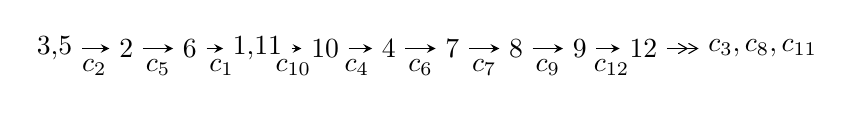
\begin{tikzpicture}[x=23pt, y=7pt]
	% node
	\node (A0) at (-1/8, 0) {3,5};
	\node (A1) at (1, 0) {2};
	\node (A2) at (2, 0) {6};
	\node (A3) at (49/16, 0) {1,11};
	\node (A4) at (33/8, 0) {10};
	\node (A5) at (41/8, 0) {4};
	\node (A6) at (49/8, 0) {7};
	\node (A7) at (57/8, 0) {8};
	\node (A8) at (65/8, 0) {9};
	\node (A9) at (73/8, 0) {12};
	\node (C1) at (1/2, -1) {$c_{2}$};
	\node (C2) at (3/2, -1) {$c_{5}$};
	\node (C3) at (5/2, -1) {$c_{1}$};
	\node (C4) at (29/8, -1) {$c_{10}$};
	\node (C5) at (37/8, -1) {$c_{4}$};
	\node (C6) at (45/8, -1) {$c_{6}$};
	\node (C7) at (53/8, -1) {$c_{7}$};
	\node (C8) at (61/8, -1) {$c_{9}$};
	\node (C9) at (69/8, -1) {$c_{12}$};
	\node (A10) at (11, 0) {$c_{3},c_{8},c_{11}$};

	% edge
	\draw[->,>=stealth]	
	(A0) edge (A1) (A1) edge (A2) (A2) edge (A3) (A3) edge (A4) (A4) edge (A5) (A5) edge (A6) (A6) edge (A7) (A7) edge (A8) (A8) edge (A9) ;
	\draw[->>,>={angle 60}]	
	(A9) edge (A10);
\end{tikzpicture} \\ 

\end{tabular} \\

\footnotetext{
The image of knot diagram is generated by the software ``\textbf{Draw programme}" developed by Andrew Bartholomew(\url{http://www.layer8.co.uk/maths/draw/index.htm\#Running-draw}), where we modified some parts for our purpose(\url{https://github.com/CATsTAILs/LinksPainter}).
}\phantom \\ \newline 
\centering \textbf{Ideals for irreducible components\footnotemark of $X_{\text{par}}$} 
 
\begin{align*}
I^u_{1}&=\langle 
47 u^{14}+142 u^{13}+\cdots+256 b+305,\;49 u^{14}+88 u^{13}+\cdots+64 a+45,\;u^{15}+u^{14}+\cdots+4 u+1\rangle \\
I^u_{2}&=\langle 
- a^4 u- a^4+a^3 u+a^3-2 a^2 u-2 a^2+a u+b- u-1,\;a^5- a^4+2 a^3- a^2+a-1,\;u^2+1\rangle \\
I^u_{3}&=\langle 
10 u^5+9 u^4-4 u^3+144 u^2+107 b-160 u+346,\\
\phantom{I^u_{3}}&\phantom{= \langle  }92 u^5-174 u^4+648 u^3-965 u^2+1819 a+1310 u-733,\;u^6-3 u^5+10 u^4-14 u^3+22 u^2-10 u+17\rangle \\
I^u_{4}&=\langle 
2 b-1,\;a,\;u+1\rangle \\
\\
\end{align*}
\raggedright * 4 irreducible components of $\dim_{\mathbb{C}}=0$, with total 32 representations.\\
\footnotetext{All coefficients of polynomials are rational numbers. But the coefficients are sometimes approximated in decimal forms when there is not enough margin.}
\newpage
\renewcommand{\arraystretch}{1}
\centering \section*{I. $I^u_{1}= \langle 47 u^{14}+142 u^{13}+\cdots+256 b+305,\;49 u^{14}+88 u^{13}+\cdots+64 a+45,\;u^{15}+u^{14}+\cdots+4 u+1 \rangle$}
\flushleft \textbf{(i) Arc colorings}\\
\begin{tabular}{m{7pt} m{180pt} m{7pt} m{180pt} }
\flushright $a_{3}=$&$\begin{pmatrix}1\\0\end{pmatrix}$ \\
\flushright $a_{5}=$&$\begin{pmatrix}0\\u\end{pmatrix}$ \\
\flushright $a_{2}=$&$\begin{pmatrix}1\\u^2\end{pmatrix}$ \\
\flushright $a_{6}=$&$\begin{pmatrix}u\\u^3+u\end{pmatrix}$ \\
\flushright $a_{1}=$&$\begin{pmatrix}u^2+1\\u^2\end{pmatrix}$ \\
\flushright $a_{11}=$&$\begin{pmatrix}-0.765625 u^{14}-1.37500 u^{13}+\cdots-8.10938 u-0.703125\\-0.183594 u^{14}-0.554688 u^{13}+\cdots-6.01953 u-1.19141\end{pmatrix}$ \\
\flushright $a_{10}=$&$\begin{pmatrix}-0.765625 u^{14}-1.37500 u^{13}+\cdots-8.10938 u-0.703125\\0.238281 u^{14}-0.0546875 u^{13}+\cdots-2.81641 u-0.582031\end{pmatrix}$ \\
\flushright $a_{4}=$&$\begin{pmatrix}-\frac{1}{32} u^{14}-\frac{1}{32} u^{13}+\cdots-\frac{1}{32} u+1\\- u^2\end{pmatrix}$ \\
\flushright $a_{7}=$&$\begin{pmatrix}\frac{1}{32} u^{13}+\frac{1}{32} u^{12}+\cdots+\frac{17}{8} u+\frac{1}{32}\\u\end{pmatrix}$ \\
\flushright $a_{8}=$&$\begin{pmatrix}\frac{1}{32} u^{13}+\frac{1}{32} u^{12}+\cdots+\frac{25}{8} u+\frac{1}{32}\\u\end{pmatrix}$ \\
\flushright $a_{9}=$&$\begin{pmatrix}-1.42188 u^{14}-1.21875 u^{13}+\cdots-2.07813 u+1.29688\\-0.230469 u^{14}-0.210938 u^{13}+\cdots-2.34766 u+0.0429688\end{pmatrix}$ \\
\flushright $a_{12}=$&$\begin{pmatrix}-0.0312500 u^{14}-0.500000 u^{13}+\cdots+0.593750 u+1.15625\\-0.0351563 u^{14}-0.320313 u^{13}+\cdots-3.38672 u-0.589844\end{pmatrix}$\\&\end{tabular}
\flushleft \textbf{(ii) Obstruction class $= -1$}\\~\\
\flushleft \textbf{(iii) Cusp Shapes $= \frac{1851}{512} u^{14}+\frac{499}{256} u^{13}+\cdots+\frac{2553}{512} u+\frac{5749}{512}$}\\~\\
\newpage\renewcommand{\arraystretch}{1}
\flushleft \textbf{(iv) u-Polynomials at the component}\newline \\
\begin{tabular}{m{50pt}|m{274pt}}
Crossings & \hspace{64pt}u-Polynomials at each crossing \\
\hline $$\begin{aligned}c_{1}\end{aligned}$$&$\begin{aligned}
&u^{15}+27 u^{14}+\cdots-10 u-1
\end{aligned}$\\
\hline $$\begin{aligned}c_{2},c_{3},c_{5}\\c_{6},c_{7}\end{aligned}$$&$\begin{aligned}
&u^{15}- u^{14}+\cdots+4 u-1
\end{aligned}$\\
\hline $$\begin{aligned}c_{4},c_{10}\end{aligned}$$&$\begin{aligned}
&u^{15}-3 u^{14}+\cdots+18 u-8
\end{aligned}$\\
\hline $$\begin{aligned}c_{8},c_{11},c_{12}\end{aligned}$$&$\begin{aligned}
&u^{15}+2 u^{14}+\cdots+13 u-4
\end{aligned}$\\
\hline $$\begin{aligned}c_{9}\end{aligned}$$&$\begin{aligned}
&u^{15}-3 u^{14}+\cdots+244 u-64
\end{aligned}$\\
\hline
\end{tabular}\\~\\
\newpage\renewcommand{\arraystretch}{1}
\flushleft \textbf{(v) Riley Polynomials at the component}\newline \\
\begin{tabular}{m{50pt}|m{274pt}}
Crossings & \hspace{64pt}Riley Polynomials at each crossing \\
\hline $$\begin{aligned}c_{1}\end{aligned}$$&$\begin{aligned}
&y^{15}-105 y^{14}+\cdots+150 y-1
\end{aligned}$\\
\hline $$\begin{aligned}c_{2},c_{3},c_{5}\\c_{6},c_{7}\end{aligned}$$&$\begin{aligned}
&y^{15}+27 y^{14}+\cdots-10 y-1
\end{aligned}$\\
\hline $$\begin{aligned}c_{4},c_{10}\end{aligned}$$&$\begin{aligned}
&y^{15}-3 y^{14}+\cdots+244 y-64
\end{aligned}$\\
\hline $$\begin{aligned}c_{8},c_{11},c_{12}\end{aligned}$$&$\begin{aligned}
&y^{15}-12 y^{14}+\cdots+209 y-16
\end{aligned}$\\
\hline $$\begin{aligned}c_{9}\end{aligned}$$&$\begin{aligned}
&y^{15}+65 y^{14}+\cdots+27664 y-4096
\end{aligned}$\\
\hline
\end{tabular}\\~\\
\newpage\flushleft \textbf{(vi) Complex Volumes and Cusp Shapes}
$$\begin{array}{c|c|c}  
\text{Solutions to }I^u_{1}& \I (\text{vol} + \sqrt{-1}CS) & \text{Cusp shape}\\
 \hline 
\begin{aligned}
u &= -1.085190 + 0.639113 I \\
a &= -0.187470 - 0.679349 I \\
b &= \phantom{-}0.244487 - 0.095273 I\end{aligned}
 & \phantom{-}3.76428 + 0.87599 I & \phantom{-}12.27688 - 4.04131 I \\ \hline\begin{aligned}
u &= -1.085190 - 0.639113 I \\
a &= -0.187470 + 0.679349 I \\
b &= \phantom{-}0.244487 + 0.095273 I\end{aligned}
 & \phantom{-}3.76428 - 0.87599 I & \phantom{-}12.27688 + 4.04131 I \\ \hline\begin{aligned}
u &= -0.171837 + 0.650095 I \\
a &= \phantom{-}1.10255 + 1.42436 I \\
b &= \phantom{-}0.682015 + 0.663583 I\end{aligned}
 & \phantom{-}3.90578 - 5.04152 I & \phantom{-}15.1629 + 7.2560 I \\ \hline\begin{aligned}
u &= -0.171837 - 0.650095 I \\
a &= \phantom{-}1.10255 - 1.42436 I \\
b &= \phantom{-}0.682015 - 0.663583 I\end{aligned}
 & \phantom{-}3.90578 + 5.04152 I & \phantom{-}15.1629 - 7.2560 I \\ \hline\begin{aligned}
u &= -0.113165 + 0.510319 I \\
a &= -1.23811 - 1.27126 I \\
b &= -0.714447 - 0.300419 I\end{aligned}
 & -1.07843 - 2.01114 I & \phantom{-}7.99911 + 6.03699 I \\ \hline\begin{aligned}
u &= -0.113165 - 0.510319 I \\
a &= -1.23811 + 1.27126 I \\
b &= -0.714447 + 0.300419 I\end{aligned}
 & -1.07843 + 2.01114 I & \phantom{-}7.99911 - 6.03699 I \\ \hline\begin{aligned}
u &= \phantom{-}0.139618 + 0.358203 I \\
a &= \phantom{-}1.15825 + 1.37391 I \\
b &= \phantom{-}0.824625 - 0.322737 I\end{aligned}
 & \phantom{-}1.56037 + 0.76584 I & \phantom{-}8.88156 - 1.45117 I \\ \hline\begin{aligned}
u &= \phantom{-}0.139618 - 0.358203 I \\
a &= \phantom{-}1.15825 - 1.37391 I \\
b &= \phantom{-}0.824625 + 0.322737 I\end{aligned}
 & \phantom{-}1.56037 - 0.76584 I & \phantom{-}8.88156 + 1.45117 I \\ \hline\begin{aligned}
u &= -0.301931\phantom{ +0.000000I} \\
a &= \phantom{-}1.66090\phantom{ +0.000000I} \\
b &= \phantom{-}0.268883\phantom{ +0.000000I}\end{aligned}
 & \phantom{-}0.626145\phantom{ +0.000000I} & \phantom{-}16.4510\phantom{ +0.000000I} \\ \hline\begin{aligned}
u &= \phantom{-}0.61910 + 1.98975 I \\
a &= -0.734091 + 0.400986 I \\
b &= -2.19546 + 0.22693 I\end{aligned}
 & -16.5790 + 11.3907 I & \phantom{-}8.72673 - 4.72209 I\\
 \hline 
 \end{array}$$\newpage$$\begin{array}{c|c|c}  
\text{Solutions to }I^u_{1}& \I (\text{vol} + \sqrt{-1}CS) & \text{Cusp shape}\\
 \hline 
\begin{aligned}
u &= \phantom{-}0.61910 - 1.98975 I \\
a &= -0.734091 - 0.400986 I \\
b &= -2.19546 - 0.22693 I\end{aligned}
 & -16.5790 - 11.3907 I & \phantom{-}8.72673 + 4.72209 I \\ \hline\begin{aligned}
u &= -0.10073 + 2.21378 I \\
a &= -0.558378 + 0.607390 I \\
b &= -1.76407 + 0.10317 I\end{aligned}
 & -16.6861 - 2.0181 I & \phantom{-}8.39824 + 0.80099 I \\ \hline\begin{aligned}
u &= -0.10073 - 2.21378 I \\
a &= -0.558378 - 0.607390 I \\
b &= -1.76407 - 0.10317 I\end{aligned}
 & -16.6861 + 2.0181 I & \phantom{-}8.39824 - 0.80099 I \\ \hline\begin{aligned}
u &= \phantom{-}0.36316 + 2.28705 I \\
a &= \phantom{-}0.626797 - 0.473627 I \\
b &= \phantom{-}2.03841 - 0.08740 I\end{aligned}
 & \phantom{-}18.2203 + 4.7904 I & \phantom{-}6.45412 - 1.91248 I \\ \hline\begin{aligned}
u &= \phantom{-}0.36316 - 2.28705 I \\
a &= \phantom{-}0.626797 + 0.473627 I \\
b &= \phantom{-}2.03841 + 0.08740 I\end{aligned}
 & \phantom{-}18.2203 - 4.7904 I & \phantom{-}6.45412 + 1.91248 I\\
 \hline 
 \end{array}$$\newpage\newpage\renewcommand{\arraystretch}{1}
\centering \section*{II. $I^u_{2}= \langle - a^4 u+a^3 u+\cdots-2 a^2-1,\;a^5- a^4+2 a^3- a^2+a-1,\;u^2+1 \rangle$}
\flushleft \textbf{(i) Arc colorings}\\
\begin{tabular}{m{7pt} m{180pt} m{7pt} m{180pt} }
\flushright $a_{3}=$&$\begin{pmatrix}1\\0\end{pmatrix}$ \\
\flushright $a_{5}=$&$\begin{pmatrix}0\\u\end{pmatrix}$ \\
\flushright $a_{2}=$&$\begin{pmatrix}1\\-1\end{pmatrix}$ \\
\flushright $a_{6}=$&$\begin{pmatrix}u\\0\end{pmatrix}$ \\
\flushright $a_{1}=$&$\begin{pmatrix}0\\-1\end{pmatrix}$ \\
\flushright $a_{11}=$&$\begin{pmatrix}a\\a^4 u+a^4- a^3 u- a^3+2 a^2 u+2 a^2- a u+u+1\end{pmatrix}$ \\
\flushright $a_{10}=$&$\begin{pmatrix}a\\a^4 u+a^4- a^3 u- a^3+2 a^2 u+2 a^2- a u- a+u+1\end{pmatrix}$ \\
\flushright $a_{4}=$&$\begin{pmatrix}- a^2 u\\1\end{pmatrix}$ \\
\flushright $a_{7}=$&$\begin{pmatrix}- a^2+u\\- u\end{pmatrix}$ \\
\flushright $a_{8}=$&$\begin{pmatrix}- a^2\\- u\end{pmatrix}$ \\
\flushright $a_{9}=$&$\begin{pmatrix}a^3+a\\a^4 u+a^4- a^3 u+2 a^2 u+2 a^2+u+1\end{pmatrix}$ \\
\flushright $a_{12}=$&$\begin{pmatrix}a^4- a^3+a^2+1\\a^4 u+a^4- a^3+2 a^2 u+2 a^2+u+1\end{pmatrix}$\\&\end{tabular}
\flushleft \textbf{(ii) Obstruction class $= 1$}\\~\\
\flushleft \textbf{(iii) Cusp Shapes $= -4 a^3+4 a^2-4 a+8$}\\~\\
\newpage\renewcommand{\arraystretch}{1}
\flushleft \textbf{(iv) u-Polynomials at the component}\newline \\
\begin{tabular}{m{50pt}|m{274pt}}
Crossings & \hspace{64pt}u-Polynomials at each crossing \\
\hline $$\begin{aligned}c_{1}\end{aligned}$$&$\begin{aligned}
&(u-1)^{10}
\end{aligned}$\\
\hline $$\begin{aligned}c_{2},c_{3},c_{5}\\c_{6},c_{7}\end{aligned}$$&$\begin{aligned}
&(u^2+1)^5
\end{aligned}$\\
\hline $$\begin{aligned}c_{4},c_{10}\end{aligned}$$&$\begin{aligned}
&u^{10}-3 u^8+4 u^6- u^4- u^2+1
\end{aligned}$\\
\hline $$\begin{aligned}c_{8}\end{aligned}$$&$\begin{aligned}
&(u^5- u^4-2 u^3+u^2+u+1)^2
\end{aligned}$\\
\hline $$\begin{aligned}c_{9}\end{aligned}$$&$\begin{aligned}
&(u^5+3 u^4+4 u^3+u^2- u-1)^2
\end{aligned}$\\
\hline $$\begin{aligned}c_{11},c_{12}\end{aligned}$$&$\begin{aligned}
&(u^5+u^4-2 u^3- u^2+u-1)^2
\end{aligned}$\\
\hline
\end{tabular}\\~\\
\newpage\renewcommand{\arraystretch}{1}
\flushleft \textbf{(v) Riley Polynomials at the component}\newline \\
\begin{tabular}{m{50pt}|m{274pt}}
Crossings & \hspace{64pt}Riley Polynomials at each crossing \\
\hline $$\begin{aligned}c_{1}\end{aligned}$$&$\begin{aligned}
&(y-1)^{10}
\end{aligned}$\\
\hline $$\begin{aligned}c_{2},c_{3},c_{5}\\c_{6},c_{7}\end{aligned}$$&$\begin{aligned}
&(y+1)^{10}
\end{aligned}$\\
\hline $$\begin{aligned}c_{4},c_{10}\end{aligned}$$&$\begin{aligned}
&(y^5-3 y^4+4 y^3- y^2- y+1)^2
\end{aligned}$\\
\hline $$\begin{aligned}c_{8},c_{11},c_{12}\end{aligned}$$&$\begin{aligned}
&(y^5-5 y^4+8 y^3-3 y^2- y-1)^2
\end{aligned}$\\
\hline $$\begin{aligned}c_{9}\end{aligned}$$&$\begin{aligned}
&(y^5- y^4+8 y^3-3 y^2+3 y-1)^2
\end{aligned}$\\
\hline
\end{tabular}\\~\\
\newpage\flushleft \textbf{(vi) Complex Volumes and Cusp Shapes}
$$\begin{array}{c|c|c}  
\text{Solutions to }I^u_{2}& \I (\text{vol} + \sqrt{-1}CS) & \text{Cusp shape}\\
 \hline 
\begin{aligned}
u &= \phantom{-0.000000 -}1.000000 I \\
a &= -0.339110 + 0.822375 I \\
b &= \phantom{-}0.271616 - 0.645450 I\end{aligned}
 & -2.96077 + 1.53058 I & \phantom{-}4.51511 - 4.43065 I \\ \hline\begin{aligned}
u &= \phantom{-0.000000 -}1.000000 I \\
a &= -0.339110 - 0.822375 I \\
b &= -1.80694 - 0.21165 I\end{aligned}
 & -2.96077 - 1.53058 I & \phantom{-}4.51511 + 4.43065 I \\ \hline\begin{aligned}
u &= \phantom{-0.000000 -}1.000000 I \\
a &= \phantom{-}0.766826\phantom{ +0.000000I} \\
b &= \phantom{-}2.07090 + 1.30408 I\end{aligned}
 & -0.888787\phantom{ +0.000000I} & \phantom{-}5.48110\phantom{ +0.000000I} \\ \hline\begin{aligned}
u &= \phantom{-0.000000 -}1.000000 I \\
a &= \phantom{-}0.455697 + 1.200150 I \\
b &= \phantom{-}1.46044 + 0.74843 I\end{aligned}
 & \phantom{-}2.58269 - 4.40083 I & \phantom{-}8.74431 + 3.49859 I \\ \hline\begin{aligned}
u &= \phantom{-0.000000 -}1.000000 I \\
a &= \phantom{-}0.455697 - 1.200150 I \\
b &= \phantom{-}0.003972 - 0.195404 I\end{aligned}
 & \phantom{-}2.58269 + 4.40083 I & \phantom{-}8.74431 - 3.49859 I \\ \hline\begin{aligned}
u &= \phantom{-0.000000 } -1.000000 I \\
a &= -0.339110 + 0.822375 I \\
b &= -1.80694 + 0.21165 I\end{aligned}
 & -2.96077 + 1.53058 I & \phantom{-}4.51511 - 4.43065 I \\ \hline\begin{aligned}
u &= \phantom{-0.000000 } -1.000000 I \\
a &= -0.339110 - 0.822375 I \\
b &= \phantom{-}0.271616 + 0.645450 I\end{aligned}
 & -2.96077 - 1.53058 I & \phantom{-}4.51511 + 4.43065 I \\ \hline\begin{aligned}
u &= \phantom{-0.000000 } -1.000000 I \\
a &= \phantom{-}0.766826\phantom{ +0.000000I} \\
b &= \phantom{-}2.07090 - 1.30408 I\end{aligned}
 & -0.888787\phantom{ +0.000000I} & \phantom{-}5.48110\phantom{ +0.000000I} \\ \hline\begin{aligned}
u &= \phantom{-0.000000 } -1.000000 I \\
a &= \phantom{-}0.455697 + 1.200150 I \\
b &= \phantom{-}0.003972 + 0.195404 I\end{aligned}
 & \phantom{-}2.58269 - 4.40083 I & \phantom{-}8.74431 + 3.49859 I \\ \hline\begin{aligned}
u &= \phantom{-0.000000 } -1.000000 I \\
a &= \phantom{-}0.455697 - 1.200150 I \\
b &= \phantom{-}1.46044 - 0.74843 I\end{aligned}
 & \phantom{-}2.58269 + 4.40083 I & \phantom{-}8.74431 - 3.49859 I\\
 \hline 
 \end{array}$$\newpage\newpage\renewcommand{\arraystretch}{1}
\centering \section*{III. $I^u_{3}= \langle 10 u^5+9 u^4+\cdots+107 b+346,\;92 u^5-174 u^4+\cdots+1819 a-733,\;u^6-3 u^5+10 u^4-14 u^3+22 u^2-10 u+17 \rangle$}
\flushleft \textbf{(i) Arc colorings}\\
\begin{tabular}{m{7pt} m{180pt} m{7pt} m{180pt} }
\flushright $a_{3}=$&$\begin{pmatrix}1\\0\end{pmatrix}$ \\
\flushright $a_{5}=$&$\begin{pmatrix}0\\u\end{pmatrix}$ \\
\flushright $a_{2}=$&$\begin{pmatrix}1\\u^2\end{pmatrix}$ \\
\flushright $a_{6}=$&$\begin{pmatrix}u\\u^3+u\end{pmatrix}$ \\
\flushright $a_{1}=$&$\begin{pmatrix}u^2+1\\u^2\end{pmatrix}$ \\
\flushright $a_{11}=$&$\begin{pmatrix}-0.0505772 u^{5}+0.0956570 u^{4}+\cdots-0.720176 u+0.402969\\-0.0934579 u^{5}-0.0841121 u^{4}+\cdots+1.49533 u-3.23364\end{pmatrix}$ \\
\flushright $a_{10}=$&$\begin{pmatrix}-0.0505772 u^{5}+0.0956570 u^{4}+\cdots-0.720176 u+0.402969\\-0.112150 u^{5}+0.299065 u^{4}+\cdots+1.79439 u-2.28037\end{pmatrix}$ \\
\flushright $a_{4}=$&$\begin{pmatrix}-0.0170423 u^{5}-0.0329852 u^{4}+\cdots+0.213854 u-0.483782\\-0.0280374 u^{5}+0.0747664 u^{4}+\cdots-0.551402 u+2.42991\end{pmatrix}$ \\
\flushright $a_{7}=$&$\begin{pmatrix}0.0588235 u^{5}-0.176471 u^{4}+\cdots+1.29412 u-0.588235\\-0.0841121 u^{5}+0.224299 u^{4}+\cdots-1.65421 u+0.289720\end{pmatrix}$ \\
\flushright $a_{8}=$&$\begin{pmatrix}-0.0252886 u^{5}+0.0478285 u^{4}+\cdots-0.360088 u-0.298516\\-0.0841121 u^{5}+0.224299 u^{4}+\cdots-1.65421 u+0.289720\end{pmatrix}$ \\
\flushright $a_{9}=$&$\begin{pmatrix}-0.109951 u^{5}+0.0775151 u^{4}+\cdots-0.652556 u+0.136888\\-0.149533 u^{5}+0.0654206 u^{4}+\cdots+1.39252 u-2.37383\end{pmatrix}$ \\
\flushright $a_{12}=$&$\begin{pmatrix}0.0340847 u^{5}+0.0659703 u^{4}+\cdots-0.427708 u+0.967565\\u-2\end{pmatrix}$\\&\end{tabular}
\flushleft \textbf{(ii) Obstruction class $= -1$}\\~\\
\flushleft \textbf{(iii) Cusp Shapes $= \frac{60}{107} u^5-\frac{160}{107} u^4+\frac{404}{107} u^3-\frac{420}{107} u^2+\frac{324}{107} u+\frac{1006}{107}$}\\~\\
\newpage\renewcommand{\arraystretch}{1}
\flushleft \textbf{(iv) u-Polynomials at the component}\newline \\
\begin{tabular}{m{50pt}|m{274pt}}
Crossings & \hspace{64pt}u-Polynomials at each crossing \\
\hline $$\begin{aligned}c_{1}\end{aligned}$$&$\begin{aligned}
&u^6+11 u^5+60 u^4+218 u^3+544 u^2+648 u+289
\end{aligned}$\\
\hline $$\begin{aligned}c_{2},c_{3},c_{5}\\c_{6},c_{7}\end{aligned}$$&$\begin{aligned}
&u^6+3 u^5+10 u^4+14 u^3+22 u^2+10 u+17
\end{aligned}$\\
\hline $$\begin{aligned}c_{4},c_{10}\end{aligned}$$&$\begin{aligned}
&(u^3+u^2+2 u+1)^2
\end{aligned}$\\
\hline $$\begin{aligned}c_{8},c_{11},c_{12}\end{aligned}$$&$\begin{aligned}
&(u^3+u^2-1)^2
\end{aligned}$\\
\hline $$\begin{aligned}c_{9}\end{aligned}$$&$\begin{aligned}
&(u^3+3 u^2+2 u-1)^2
\end{aligned}$\\
\hline
\end{tabular}\\~\\
\newpage\renewcommand{\arraystretch}{1}
\flushleft \textbf{(v) Riley Polynomials at the component}\newline \\
\begin{tabular}{m{50pt}|m{274pt}}
Crossings & \hspace{64pt}Riley Polynomials at each crossing \\
\hline $$\begin{aligned}c_{1}\end{aligned}$$&$\begin{aligned}
&y^6- y^5-108 y^4+4078 y^3+48088 y^2-105472 y+83521
\end{aligned}$\\
\hline $$\begin{aligned}c_{2},c_{3},c_{5}\\c_{6},c_{7}\end{aligned}$$&$\begin{aligned}
&y^6+11 y^5+60 y^4+218 y^3+544 y^2+648 y+289
\end{aligned}$\\
\hline $$\begin{aligned}c_{4},c_{10}\end{aligned}$$&$\begin{aligned}
&(y^3+3 y^2+2 y-1)^2
\end{aligned}$\\
\hline $$\begin{aligned}c_{8},c_{11},c_{12}\end{aligned}$$&$\begin{aligned}
&(y^3- y^2+2 y-1)^2
\end{aligned}$\\
\hline $$\begin{aligned}c_{9}\end{aligned}$$&$\begin{aligned}
&(y^3-5 y^2+10 y-1)^2
\end{aligned}$\\
\hline
\end{tabular}\\~\\
\newpage\flushleft \textbf{(vi) Complex Volumes and Cusp Shapes}
$$\begin{array}{c|c|c}  
\text{Solutions to }I^u_{3}& \I (\text{vol} + \sqrt{-1}CS) & \text{Cusp shape}\\
 \hline 
\begin{aligned}
u &= -0.162359 + 1.038790 I \\
a &= -0.083694 - 0.535481 I \\
b &= -2.03980 + 1.82295 I\end{aligned}
 & -2.17641\phantom{ +0.000000I} & \phantom{-}13.01951 + 0. I\phantom{ +0.000000I} \\ \hline\begin{aligned}
u &= -0.162359 - 1.038790 I \\
a &= -0.083694 + 0.535481 I \\
b &= -2.03980 - 1.82295 I\end{aligned}
 & -2.17641\phantom{ +0.000000I} & \phantom{-}13.01951 + 0. I\phantom{ +0.000000I} \\ \hline\begin{aligned}
u &= \phantom{-}1.23597 + 1.45071 I \\
a &= \phantom{-}0.595267 + 0.358893 I \\
b &= \phantom{-}1.109500 + 0.002038 I\end{aligned}
 & -6.31400 + 2.82812 I & \phantom{-}6.49024 - 2.97945 I \\ \hline\begin{aligned}
u &= \phantom{-}1.23597 - 1.45071 I \\
a &= \phantom{-}0.595267 - 0.358893 I \\
b &= \phantom{-}1.109500 - 0.002038 I\end{aligned}
 & -6.31400 - 2.82812 I & \phantom{-}6.49024 + 2.97945 I \\ \hline\begin{aligned}
u &= \phantom{-}0.42639 + 2.01299 I \\
a &= -0.599808 - 0.233897 I \\
b &= -1.56970 - 0.18054 I\end{aligned}
 & -6.31400 - 2.82812 I & \phantom{-}6.49024 + 2.97945 I \\ \hline\begin{aligned}
u &= \phantom{-}0.42639 - 2.01299 I \\
a &= -0.599808 + 0.233897 I \\
b &= -1.56970 + 0.18054 I\end{aligned}
 & -6.31400 + 2.82812 I & \phantom{-}6.49024 - 2.97945 I\\
 \hline 
 \end{array}$$\newpage\newpage\renewcommand{\arraystretch}{1}
\centering \section*{IV. $I^u_{4}= \langle 2 b-1,\;a,\;u+1 \rangle$}
\flushleft \textbf{(i) Arc colorings}\\
\begin{tabular}{m{7pt} m{180pt} m{7pt} m{180pt} }
\flushright $a_{3}=$&$\begin{pmatrix}1\\0\end{pmatrix}$ \\
\flushright $a_{5}=$&$\begin{pmatrix}0\\-1\end{pmatrix}$ \\
\flushright $a_{2}=$&$\begin{pmatrix}1\\1\end{pmatrix}$ \\
\flushright $a_{6}=$&$\begin{pmatrix}-1\\-2\end{pmatrix}$ \\
\flushright $a_{1}=$&$\begin{pmatrix}2\\1\end{pmatrix}$ \\
\flushright $a_{11}=$&$\begin{pmatrix}0\\0.5\end{pmatrix}$ \\
\flushright $a_{10}=$&$\begin{pmatrix}0\\0.5\end{pmatrix}$ \\
\flushright $a_{4}=$&$\begin{pmatrix}0\\-1\end{pmatrix}$ \\
\flushright $a_{7}=$&$\begin{pmatrix}-1\\-1\end{pmatrix}$ \\
\flushright $a_{8}=$&$\begin{pmatrix}-2\\-1\end{pmatrix}$ \\
\flushright $a_{9}=$&$\begin{pmatrix}0\\0.5\end{pmatrix}$ \\
\flushright $a_{12}=$&$\begin{pmatrix}2\\1.5\end{pmatrix}$\\&\end{tabular}
\flushleft \textbf{(ii) Obstruction class $= 1$}\\~\\
\flushleft \textbf{(iii) Cusp Shapes $= 9.75$}\\~\\
\newpage\renewcommand{\arraystretch}{1}
\flushleft \textbf{(iv) u-Polynomials at the component}\newline \\
\begin{tabular}{m{50pt}|m{274pt}}
Crossings & \hspace{64pt}u-Polynomials at each crossing \\
\hline $$\begin{aligned}c_{1},c_{2},c_{3}\\c_{8}\end{aligned}$$&$\begin{aligned}
&u+1
\end{aligned}$\\
\hline $$\begin{aligned}c_{4},c_{9},c_{10}\end{aligned}$$&$\begin{aligned}
&u
\end{aligned}$\\
\hline $$\begin{aligned}c_{5},c_{6},c_{7}\\c_{11},c_{12}\end{aligned}$$&$\begin{aligned}
&u-1
\end{aligned}$\\
\hline
\end{tabular}\\~\\
\newpage\renewcommand{\arraystretch}{1}
\flushleft \textbf{(v) Riley Polynomials at the component}\newline \\
\begin{tabular}{m{50pt}|m{274pt}}
Crossings & \hspace{64pt}Riley Polynomials at each crossing \\
\hline $$\begin{aligned}c_{1},c_{2},c_{3}\\c_{5},c_{6},c_{7}\\c_{8},c_{11},c_{12}\end{aligned}$$&$\begin{aligned}
&y-1
\end{aligned}$\\
\hline $$\begin{aligned}c_{4},c_{9},c_{10}\end{aligned}$$&$\begin{aligned}
&y
\end{aligned}$\\
\hline
\end{tabular}\\~\\
\newpage\flushleft \textbf{(vi) Complex Volumes and Cusp Shapes}
$$\begin{array}{c|c|c}  
\text{Solutions to }I^u_{4}& \I (\text{vol} + \sqrt{-1}CS) & \text{Cusp shape}\\
 \hline 
\begin{aligned}
u &= -1.00000\phantom{ +0.000000I} \\
a &= \phantom{-0.000000 } 0 \\
b &= \phantom{-}0.500000\phantom{ +0.000000I}\end{aligned}
 & \phantom{-}3.28987\phantom{ +0.000000I} & \phantom{-}9.75000\phantom{ +0.000000I}\\
 \hline 
 \end{array}$$\newpage
\newpage\renewcommand{\arraystretch}{1}
\centering \section*{ V. u-Polynomials}
\begin{tabular}{m{50pt}|m{274pt}}
Crossings & \hspace{64pt}u-Polynomials at each crossing \\
\hline $$\begin{aligned}c_{1}\end{aligned}$$&$\begin{aligned}
&((u-1)^{10})(u+1)(u^{6}+11 u^{5}+\cdots+648 u+289)\\
&\cdot(u^{15}+27 u^{14}+\cdots-10 u-1)
\end{aligned}$\\
\hline $$\begin{aligned}c_{2},c_{3}\end{aligned}$$&$\begin{aligned}
&(u+1)(u^2+1)^5(u^6+3 u^5+10 u^4+14 u^3+22 u^2+10 u+17)\\
&\cdot(u^{15}- u^{14}+\cdots+4 u-1)
\end{aligned}$\\
\hline $$\begin{aligned}c_{4},c_{10}\end{aligned}$$&$\begin{aligned}
&u(u^3+u^2+2 u+1)^2(u^{10}-3 u^8+4 u^6- u^4- u^2+1)\\
&\cdot(u^{15}-3 u^{14}+\cdots+18 u-8)
\end{aligned}$\\
\hline $$\begin{aligned}c_{5},c_{6},c_{7}\end{aligned}$$&$\begin{aligned}
&(u-1)(u^2+1)^5(u^6+3 u^5+10 u^4+14 u^3+22 u^2+10 u+17)\\
&\cdot(u^{15}- u^{14}+\cdots+4 u-1)
\end{aligned}$\\
\hline $$\begin{aligned}c_{8}\end{aligned}$$&$\begin{aligned}
&(u+1)(u^3+u^2-1)^2(u^5- u^4-2 u^3+u^2+u+1)^2\\
&\cdot(u^{15}+2 u^{14}+\cdots+13 u-4)
\end{aligned}$\\
\hline $$\begin{aligned}c_{9}\end{aligned}$$&$\begin{aligned}
&u(u^3+3 u^2+2 u-1)^2(u^5+3 u^4+4 u^3+u^2- u-1)^2\\
&\cdot(u^{15}-3 u^{14}+\cdots+244 u-64)
\end{aligned}$\\
\hline $$\begin{aligned}c_{11},c_{12}\end{aligned}$$&$\begin{aligned}
&(u-1)(u^3+u^2-1)^2(u^5+u^4-2 u^3- u^2+u-1)^2\\
&\cdot(u^{15}+2 u^{14}+\cdots+13 u-4)
\end{aligned}$\\
\hline
\end{tabular}\newpage\renewcommand{\arraystretch}{1}
\centering \section*{ VI. Riley Polynomials}
\begin{tabular}{m{50pt}|m{274pt}}
Crossings & \hspace{64pt}Riley Polynomials at each crossing \\
\hline $$\begin{aligned}c_{1}\end{aligned}$$&$\begin{aligned}
&((y-1)^{11})(y^6- y^5+\cdots-105472 y+83521)\\
&\cdot(y^{15}-105 y^{14}+\cdots+150 y-1)
\end{aligned}$\\
\hline $$\begin{aligned}c_{2},c_{3},c_{5}\\c_{6},c_{7}\end{aligned}$$&$\begin{aligned}
&(y-1)(y+1)^{10}(y^{6}+11 y^{5}+\cdots+648 y+289)\\
&\cdot(y^{15}+27 y^{14}+\cdots-10 y-1)
\end{aligned}$\\
\hline $$\begin{aligned}c_{4},c_{10}\end{aligned}$$&$\begin{aligned}
&y(y^3+3 y^2+2 y-1)^2(y^5-3 y^4+4 y^3- y^2- y+1)^2\\
&\cdot(y^{15}-3 y^{14}+\cdots+244 y-64)
\end{aligned}$\\
\hline $$\begin{aligned}c_{8},c_{11},c_{12}\end{aligned}$$&$\begin{aligned}
&(y-1)(y^3- y^2+2 y-1)^2(y^5-5 y^4+8 y^3-3 y^2- y-1)^2\\
&\cdot(y^{15}-12 y^{14}+\cdots+209 y-16)
\end{aligned}$\\
\hline $$\begin{aligned}c_{9}\end{aligned}$$&$\begin{aligned}
&y(y^3-5 y^2+10 y-1)^2(y^5- y^4+8 y^3-3 y^2+3 y-1)^2\\
&\cdot(y^{15}+65 y^{14}+\cdots+27664 y-4096)
\end{aligned}$\\
\hline
\end{tabular}
\vskip 2pc
\end{document}